\documentclass[bachelor, och, pract]{SCWorks}
\usepackage[T2A]{fontenc}
\usepackage[utf8]{inputenc}
\usepackage{graphicx}
\usepackage[sort,compress]{cite}
\usepackage{amsmath}
\usepackage{amssymb}
\usepackage{amsthm}
\usepackage{fancyvrb}
\usepackage{longtable}
\usepackage{array}
\usepackage[english,russian]{babel}
\usepackage{minted}
\usepackage{tempora}
\usepackage{titlesec}
\usepackage[colorlinks=false]{hyperref}
\usepackage{xcolor}
\usepackage{hyperref}

\definecolor{linkcolor}{HTML}{799B03} % цвет ссылок
\definecolor{urlcolor}{HTML}{799B03} % цвет гиперссылок

\hypersetup{pdfstartview=FitH,  linkcolor=linkcolor,urlcolor=urlcolor, colorlinks=true}

\hypersetup{ %содержание
colorlinks,
citecolor=black,
filecolor=black,
linkcolor=black,
urlcolor=black
}
\theoremstyle{remark}
\newtheorem{theorem}{Теорема}
\newtheorem{definition}{Определение}
\newtheorem{comment}{Замечание}

\begin{document}
    \hfill \break
    \hfill \break
    \hfill \break
    \hfill \break
    \hfill \break
    \hfill \break
    \hfill \break
    \hfill \break
    \hfill \break
    \hfill \break
    \hfill \break
    \hfill \break
    \begin{center}
        \Huge Лекции по Операционным системам
    \end{center}
    \hfill \break
    \hfill \break
    \hfill \break
    \hfill \break
    \hfill \break
    \hfill \break
    \hfill \break
    \hfill \break
    \hfill \break

    \begin{center} Сверстал: Кузякин Никита Александрович \end{center}
    \begin{center} По лекциям ИТМО \end{center}
    \begin{center}Плейлист с лекциями "--- \href{https://www.youtube.com/watch?v=NctMiqgVRxA&list=PLBWafxh1dFuyGGcWXmR_EngRkoUWvDFJi&index=1}{тут}\end{center}
    \thispagestyle{empty} % выключаем отображение номера для этой страницы
     
    \newpage
    \tableofcontents

    \section{Архитектура компьютерных систем}

    Первоначальными двумя архитектурами компьютерных систем являются Гарвардская и Неймановская архитектуры.

    \begin{figure}[H]
        \begin{center}
            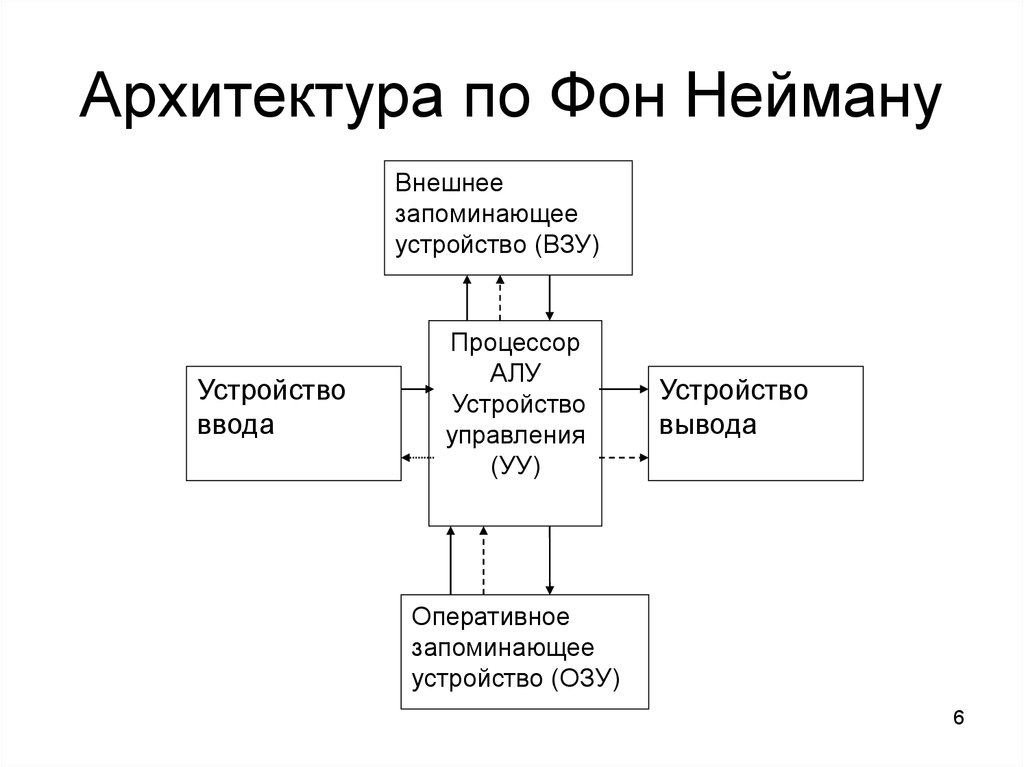
\includegraphics[scale=0.7]{res/Neumann_architecture.png}
        \end{center}
    \end{figure}

    \begin{figure}[H]
        \begin{center}
            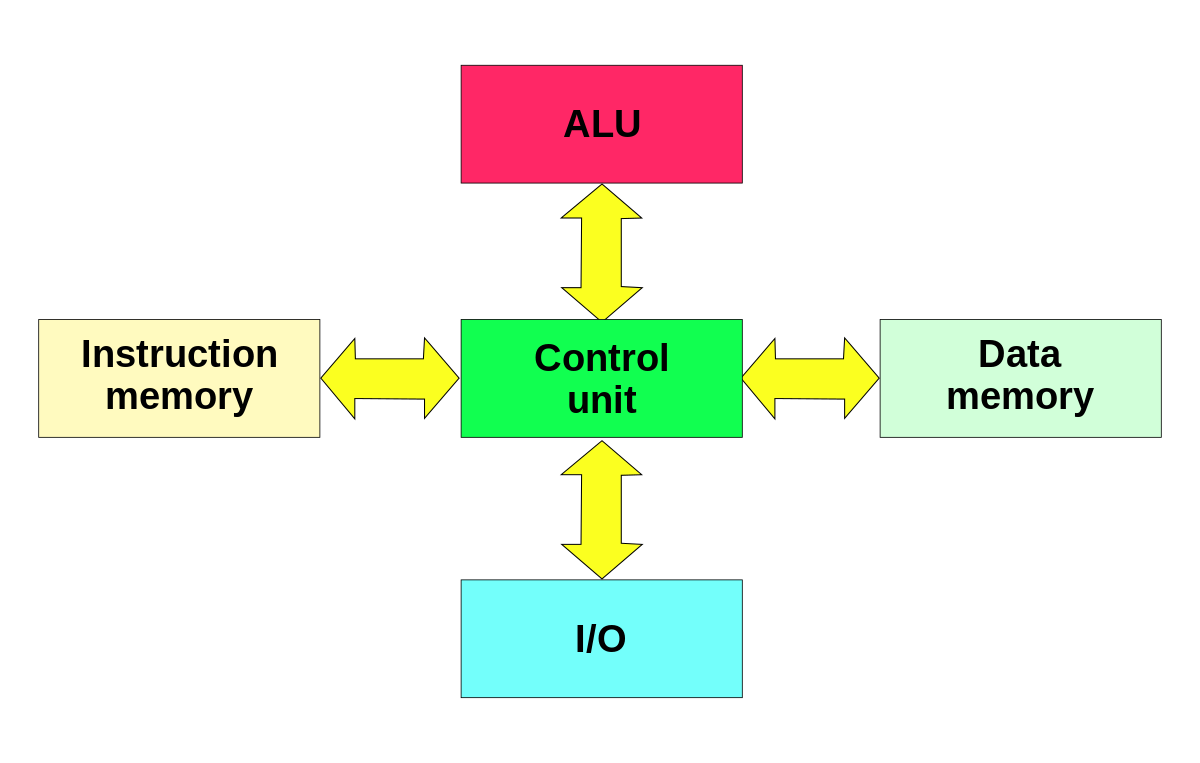
\includegraphics[scale=0.3]{res/Harvard_architecture.png}
            \caption{Гарвардская архитектура ЭВМ}
        \end{center}
    \end{figure}

    Любая вычислительная машины состоит из управляющего устройства (организует вычисления) и арифметико "= логического устройства (производит вычисление арифметических операций), а также различных видов памяти.
    
    В архитектуре фон Неймана предполагается, что есть единое управляющие устройство, память при этом общая (и данная, и программа в одно блоке).

    \textbf{Принципы архитектуры фон Неймана:} 

    \begin{itemize}[label=$\bullet$]
        \item Принцип однородности памяти "--- команды и данные хранятся в одной и той же памяти (внешне неразличимы).
        \item Принцип адресности "--- память состоит из пронумерованных ячеек, процессору доступна любая ячейка.
        \item Принцип программного управления "--- вычисления представлены в виде программы, состоящей из последовательности команд.
        \item Принцип двоичного кодирования "--- вся информация, как данные, так и команды, кодируются двоичными цифрами 0 и 1.
    \end{itemize}

    \hfill \break
    \begin{center}
        \textbf{UMA / NUMA}        
    \end{center}

    В архитектуре U\textbf{UMA} подразумевается, что все устройства являются одноранговыми. Те у любого устройства в системе равные права на доступ к памяти и системные характеристики обращения к ней. 

    \begin{figure}[H]
        \begin{center}
            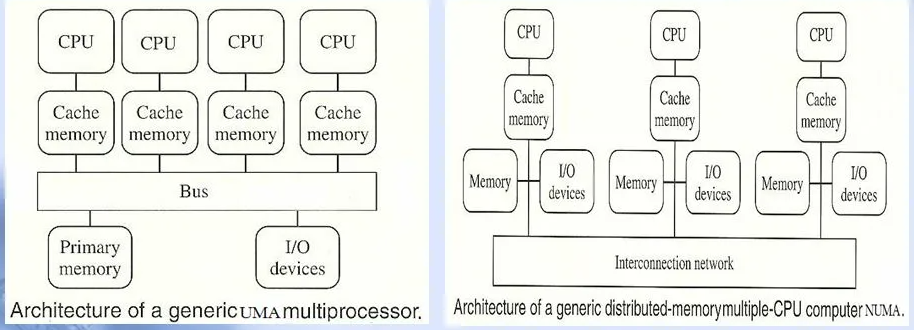
\includegraphics[scale=0.5]{res/UMA-NUMA_architecture.png}
            \caption{Гарвардская архитектура ЭВМ}
        \end{center}
    \end{figure}

    Минусом данной архитектуры является, то что тяжело организовать доступ к памяти для большого числа процессоров.

    В архитектуре \textbf{NUMA} у нас есть память, которая находится ближе к какому-то процессору и память, которая доступна через коммутатор (передает данные через порты). 

    Адресное пространство для данной архитектуры является общим.

    Огромным плюсом является, что можно заменять ее части прямо во время работы, что сильно повышает надежность системы.

    \section{Обзор элементов компьютерных систем}
    
    \subsection{Процессор}
    \begin{figure}[H]
        \begin{center}
            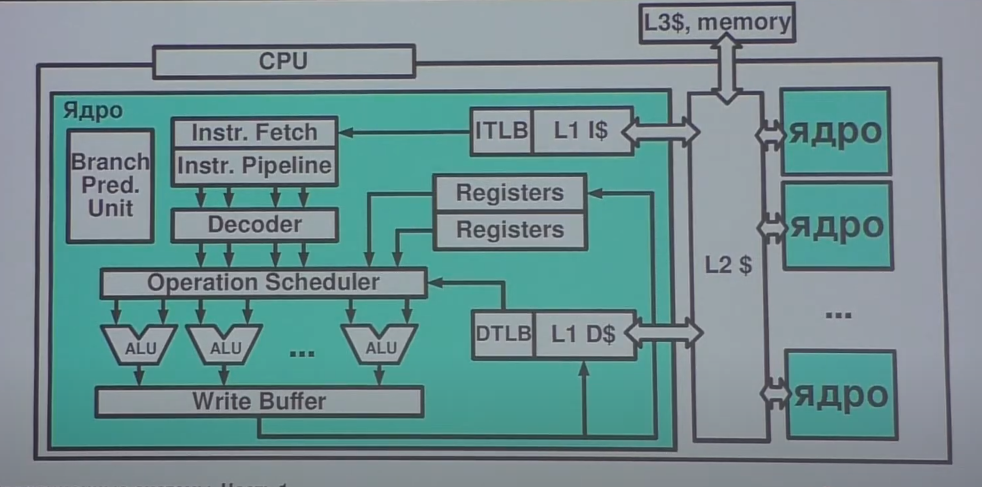
\includegraphics[scale=0.5]{res/processor.png}
        \end{center}
    \end{figure}

    Составляющие: 
    
    \begin{enumerate}
        \item Арифметико-логическое устройство (АЛУ), выполняющее действия над операндами.
        \item Буфер ассоциативной трансляции (TLB) "--- хранит информацию, есть ли такие"=то данные в данном кэше.
        \item Кэш процессора, используемый микропроцессором компьютера для уменьшения среднего времени доступа к компьютерной памяти. Делится на L1 i и L1 d. Один из них хранит набор инструкций для работы с кэшем, другой данные.
        \item Регистры для хранения данных, адресов и служебной информации.
        \item Декодер команд.
        \item Буфер для записи "--- хранит данные, пока буфер не освободится для записи.
        \item Branch Pred. Unit "--- предполагает куда будут записаны данные, по какому адресу (последовательно или с каким"=то отступом).
        \item Instr. Pipeline "--- это метод реализации параллелизма на уровне команд в пределах одного процессора.
    \end{enumerate}

    \hfill \break
    Важно помнить, что процессор выполняет команды последовательно. Пока один компонент выполняет одно действие, другой выполняет другое (они не останавливаются пока одни данные пройдут от начала до конца).

    \begin{definition}
        \textbf{Виртуальная память} "--- это подход к управлению памятью компьютером, который скрывает физическую память (в различных формах, таких как: оперативная память, ПЗУ или жесткие диски) за единым интерфейсом, позволяя создавать программы, которые работают с ними как с единым непрерывным массивом памяти с произвольным доступом.
    \end{definition}

    \begin{figure}[H]
        \begin{center}
            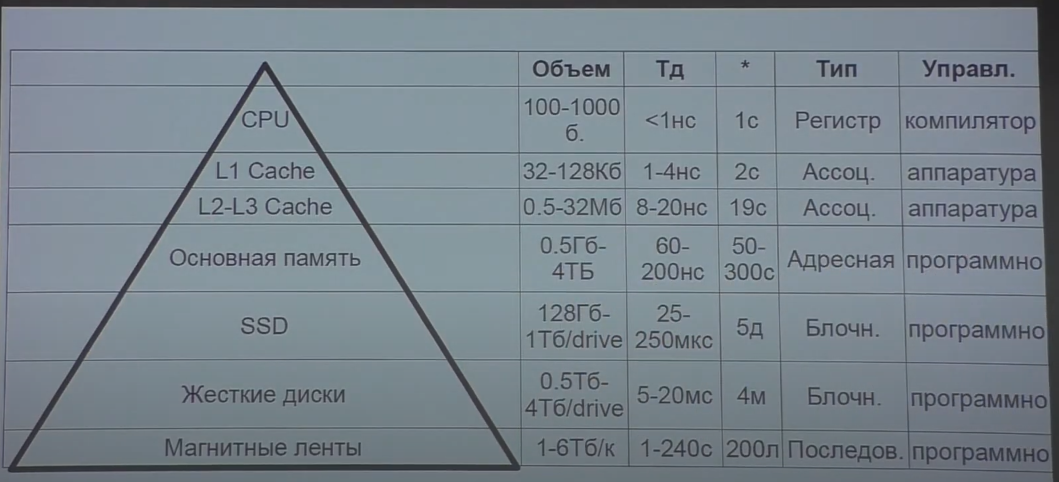
\includegraphics[scale=0.4]{res/memory-pyramid.png}
        \end{center}
    \end{figure}

    Управляется компилятором "--- означает, что именно компилятор определяет, как именно ваша программа будет взаимодействовать с данным блоком памяти, те что в какие регистры запишется и тд. 

















    \section{Полезные утилиты}

    Google Test Framework "--- \href{https://google.github.io/googletest/primer.html}{https://google.github.io/googletest/primer.html}

\end{document}